% Unofficial UofT Poster template.
% A fork of the UMich template https://www.overleaf.com/latex/templates/university-of-michigan-umich-poster-template/xpnqzzxwbjzc
% which is fork of the MSU template https://www.overleaf.com/latex/templates/an-unofficial-poster-template-for-michigan-state-university/wnymbgpxnnwd
% which is a fork of https://www.overleaf.com/latex/templates/an-unofficial-poster-template-for-new-york-university/krgqtqmzdqhg
% which is a fork of https://github.com/anishathalye/gemini
% also refer to https://github.com/k4rtik/uchicago-poster

\documentclass[final]{beamer}

% ====================
% Packages
% ====================

\usepackage[T1]{fontenc}
 \usepackage[utf8]{luainputenc}
\usepackage{lmodern}
\usepackage[size=custom, width=125,height=93, scale=1.2]{beamerposter}
\usetheme{gemini}
\usecolortheme{uoft}
\usepackage{graphicx}
\usepackage{booktabs}
\usepackage{tikz}
\usepackage{pgfplots}
\pgfplotsset{compat=1.14}
\usepackage{anyfontsize}

% ====================
% Lengths
% ====================

% If you have N columns, choose \sepwidth and \colwidth such that
% (N+1)*\sepwidth + N*\colwidth = \paperwidth
\newlength{\sepwidth}
\newlength{\colwidth}
\setlength{\sepwidth}{0.025\paperwidth}
\setlength{\colwidth}{0.3\paperwidth}

\newcommand{\separatorcolumn}{\begin{column}{\sepwidth}\end{column}}

% ====================
% Title
% ====================

\title{Analyzing Patterns of Computational Similarity between Kinase Ligands}

\author{Jack Ringer}

\institute[shortinst]{University of New Mexico}

% ====================
% Footer (optional)
% ====================

\footercontent{
  \href{https://github.com/Jack-42/https://github.com/Jack-42/ligandActivityAnalysis}{GitHub: https://github.com/Jack-42/ligandActivityAnalysis} \hfill
CFDE Summer Internship at UNM, 2025 \hfill
{johnjack0987@gmail.com}}
% (can be left out to remove footer)

% ====================
% Logo (optional)
% ====================

% use this to include logos on the left and/or right side of the header:
% Left: institution
 \logoright{
\includegraphics[height=8cm]{logos/unm_hsc.jpg}}
% Right: funding agencies and other affilations 
%\logoright{\includegraphics[height=7cm]{logos/NSF.eps}}
% ====================
% Body
% ====================

\begin{document}



\begin{frame}[t]
\begin{columns}[t]
\separatorcolumn

\begin{column}{\colwidth}

  \begin{block}{Background and Overview}
  \heading{Background}
   Protein kinases are relevant to a large number of human pathologies, including cancer, immune disorders, and infectious diseases. Protein Kinases have been classified into several different groups (a.k.a. ``families''). These classifications are based on sequence similarity, evolutionary conservation, and known functions. 

% TODO: include image of kinase family tree here

The similarity property principle (SPP), has been enormously influential in the realm of medicinal chemistry~\cite{maggiora_vogt_stumpfe_bajorath_2013}. According to the SPP, structurally-similar compounds often exhibit similar properties. Among these properties is biological activity, such that similar compounds often demonstrate similar activity. 

This work investigates whether ligands which are active within a particular kinase group are more similar to one another than kinase ligands generally. 
    \heading{Why is this important?}
    \begin{itemize}
        \item Relevant to drug discovery research
        \item If there is a relationship between kinase group and ligand similarity, then it may be informative to look at the ligands of related kinases (i.e., those belonging to the same group)
        \item There may not be much information on a particular protein target, but related and more well-studied proteins could potentially be informative
    \end{itemize}

  \end{block}

  \begin{block}{Methodology Overview}
    The set of active ligands and their relationship to specific kinase proteins/groups was determined using data from single protein target binding assays in the ChEMBL database~\cite{chembl_db_2023}. 
    \begin{itemize}
        \item Assay/ligand selection based on Pharos~\cite{pharos_2022}
        \item Remove assays where target was a variant/mutant
        \item Filtered out PAINS compounds
        \item Molecular weight of ligand must fall between [200, 900] Da
    \end{itemize}

    The criteria above resulted in a dataset with the folllowing properties:

    \begin{table}[!ht]
    \centering
    \begin{tabular}{l|l}
        \hline
        \textbf{Variable} & \textbf{Value} \\ \hline
        N. Protein Targets & 423 \\ \hline
        N. Assays & 73,487 \\ \hline
        N. Assay-Ligand Pairs & 38,622 \\ \hline
        N. Unique Ligands & 9,995 \\ \hline
    \end{tabular}
    \end{table}

    Ligands are considered active within a Kinase group if they were identified as an active within an assay targeting a protein belonging to the group. 

    After determining the set of ligands and their group relationship(s), Morgan fingerprints were computed using RDKit. Tanimoto similarity coefficients were then computed between these 2D fingerprints. 

    % TODO: include image with ligand pairs and tanimoto coeff values
  \end{block}
\end{column}

\separatorcolumn

\begin{column}{\colwidth}

  \begin{block}{Results}

    \begin{figure}
        \centering
        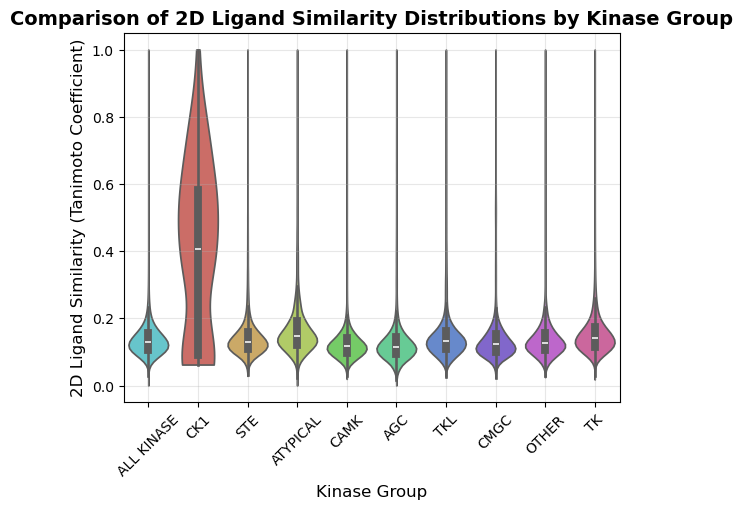
\includegraphics[width=\textwidth]{figures/violin_plot.png}
        \caption{Comparison of 2D structural similarity distributions by kinase group}
        \label{violin_plot}
    \end{figure}
 
 % TODO: include enrichment plots 
 % TODO: add dist. plots for assays and targets
 % TODO: add assay-ligand scatterplot

  \end{block}

\end{column}

\separatorcolumn

\begin{column}{\colwidth} 
  \begin{block}{Discussion}
    \heading{Limitations}
    \begin{itemize} 
        \item Only considered Morgan fingerprints + Tanimoto coefficients when measuring ``similarity'' of ligands
        \item Methodology does not account for differences in assay conditions
        \item Data gathered from ChEMBL may not reflect global trends
    \end{itemize}
    \heading{Conclusions}
      Overall, this study found no clear relationship between kinase group and 2D ligand similarity. 
  \end{block}

  \begin{block}{Acknowledgement}
  \small{
    Much thanks to my advisor Dr.~Vincent Metzger for his guidance and input over the course of this project. I'd also like to thank Dr.~Jeremy Yang, Dr.~Cristian Bologa, and Dr.~Praveen Kumar for their feedback during weekly meetings over the course of the internship. Finally, I'd like to thank the   authors of ChEMBL DB~\cite{chembl_db_2023}.}
  \end{block}

  \begin{block}{References}
    \tiny{\bibliographystyle{plain}\bibliography{poster}}
  \end{block}

\end{column}

\separatorcolumn
\end{columns}
\end{frame}

\end{document}
